\documentclass[a4paper,11pt]{scrreprt}
    %% Used for changing geometry of the page
    %% Cover page text cannot overlay cover sketching/style 
    %% https://ctan.org/pkg/geometry?lang=en
\usepackage{geometry}
    %% Changes language of some packages protocols
    %% e.g., when captioning images: Figure 1. -> Figura 1.
    %% https://ctan.org/pkg/babel?lang=en
\usepackage[portuguese]{babel}
    %% Used for special fonts
    %% Cannot be compiled with pdflatex
    %% https://ctan.org/pkg/fontspec?lang=en
\usepackage{fontspec}
    %% Arial FONT
    \setmainfont{Arial}
\usepackage{subfiles}
    %% More colors and color options
    %% https://ctan.org/pkg/xcolor?lang=en
    %% https://ctan.org/pkg/colortbl?lang=en
\usepackage{xcolor,colortbl}
    %% More tabular options, like dashed/dotted lines
    %% https://ctan.org/pkg/arydshln?lang=en
\usepackage{arydshln}
    %% List of acronyms
    %% https://ctan.org/pkg/nomencl?lang=en
\usepackage[intoc]{nomencl}
    %% Must be called to init nomencl environment  
    \makenomenclature
    %% More images options/settings
    %% https://ctan.org/pkg/graphicx?lang=en
\usepackage{graphics}
    %% Defining subdirectories to image path enviornment
    %% \graphicspath{{sub1}{sub2}...{subN}}
    \graphicspath{{images}}
    
    %% used to handle cross-referencing commands in LaTeX to produce hypertext links in the document
    %% https://ctan.org/pkg/hyperref?lang=en
\usepackage{hyperref}
    %% math environments
    %% https://ctan.org/pkg/amsmath?lang=en

    %% settings
    \hypersetup{
        colorlinks,
        citecolor=black,
        filecolor=black,
        linkcolor=black,
        urlcolor=black
    }

\usepackage{amsmath}
    %% Defining backgrouns, used to make the cover
    %% https://ctan.org/pkg/background?lang=en
\usepackage[some]{background}
    %% Used to make drawings or complex graphics
    %% http://pgf.sourceforge.net/pgf_CVS.pdf
\usepackage{tikz}
    %% Tikz library to point operations ((x1,y1) + (x2,y2))
    \usetikzlibrary{calc}
\usepackage{lscape}
%% Defining sfdefault font and default font for document
\renewcommand{\familydefault}{\sfdefault}

\usepackage{float}

\usepackage{minted}

%% Costume made cover 
%% From there you can use \makecover command to build the cover
%% Blue cover color
\definecolor{titlepagecolor}{RGB}{54,95,145}

%==========================================================================
% COLORED BAR ON THE LEFT SIDE
%==========================================================================

\backgroundsetup{
    scale=1,
    angle=0,
    opacity=1,
    contents={
            \begin{tikzpicture}[remember picture,overlay]
                \path [fill=titlepagecolor]
                (current page.north west) -- ($(current page.north west) + (5,0)$)
                -- ($(current page.south west) + (5,0)$)-- (current page.south west);
                \node[color=white] at ($(current page.south west) + (3,4)$) {\bfseries {\fontsize{50}{60} \textsf{SD}}};
                %\node[color=titlepagecolor] at ($(current page.south west) + (5.8,4)$) {\bfseries {\fontsize{120}{60} \textsf{4}}};
            \end{tikzpicture}
        }
}

%==========================================================================
% TITLE PAGE INFO
%==========================================================================

%% Changes values in this field to show information in the cover and back cover about your team/project


%% TITLE
\title{Sistema de gestão de reservas de voos}

%% AUTHORS
\author{
    \begin{tabular} { c c }
        
\includegraphics[scale=0.2]{author/marco.jpg} & 
\includegraphics[scale=0.2]{author/mariana.jpg} \\
        62608 - Marco Sousa                           & 93198 - Mariana Marques                       \\
        %\hline                                                                                        \\
        
\includegraphics[scale=0.2]{author/ze.jpg} & 
\includegraphics[scale=0.2]{author/miguel.jpg} \\
        93271 - José Malheiro                         & 94269 - Miguel Fernandes
    \end{tabular}
}

%% Date

\date{\today}

%% Course
\newcommand{\Course}{Licenciatura em Engenharia Informática}

%% Department
\newcommand{\Department}{Escola de Engenharia}

%% UniName
\newcommand{\UniName}{Universidade do Minho}

\newcommand{\UcName}{Sistemas Distribuídos}

\newcommand{\GroupId}{Grupo 12}

%% UniPic
\newcommand{\UniPic}{
\includegraphics[scale=0.09]{uminho.png}}

%% University 
\newcommand{\University}{
    \begin{flushleft}
        \UniPic
    \end{flushleft}
    \textcolor{gray}{\small\textbf{\textsf{\UniName}}}\par
    \textcolor{gray!80!white}{\small{\textsf{\Department}}}\par
    \textcolor{gray!70!white}{\small{\textsf{\Course}}}
}

%% UC
\newcommand{\UC}{
    \begin{flushleft}
        \par\textcolor{titlepagecolor}{  \LARGE\textbf{\textsf{Unidade Curricular de \\ \UcName}}}
    \end{flushleft}
}

%% School Year
\newcommand{\SchoolYear}{
    \small{\textsf{Ano Letivo de 2021/2022}}}


%% Define new command to show title, author and date
\makeatletter
\let\Title\@title
\let\Author\@author
\let\Date\@date
\makeatother

%==========================================================================
% CLASSIFICATION SECTION 
%==========================================================================

%% School Year
\newcommand{\ReceptionDate}{}
%% Responsible
\newcommand{\Responsible}{}
%% Evaluation
\newcommand{\Evaluation}{}
%% Observations
\newcommand{\Observations}{}


%% MAKETEMPLATE
\newcommand{\makecover}{

    %==========================================================================
    % BEGIN COVER PAGE 
    %==========================================================================

    %% Removes page number on footer
    \thispagestyle{empty}

    %% No indentation 
    \setlength{\parindent}{0em}

    %% Put Background defined on \backgroundsetup, in this page
    \BgThispage

    %% Changing geometry to prevent overlay with text
    %% At the end of back cover, geometry is default with \restoregeometry
    \newgeometry{top=3.5cm,left=6cm,right=3cm,bottom=2cm}

    %% builds university info defined previously
    \University
    \vspace{1cm}
    %% builds curricular unity info defined previously
    \UC
    %% builds school year info defined previously
    \SchoolYear

    \vspace*{4cm}
    %% bigger space (i think its the default one) between paragraphs 
    \setlength{\parskip}{1em}

    %% builds title info defined previously
    \par\textbf{\textsf{\huge\Title}}
    \par\textbf{\GroupId}
    \vspace{1cm}
    %% builds author(s) info defined previously
    \par\begin{center}
        \Author
    \end{center}

    \vspace{0.5cm}

    %% builds date info defined previously
    \par\Date
    \restoregeometry
    \pagebreak

    %==========================================================================
    % END COVER PAGE 
    %==========================================================================
}


\graphicspath{ {./assets/} }

% TODO
% ABSTRACT - inclui objetivos e descrição MARCO
% abordar motivo de criar passos e material
% considerações finais

\begin{document}

\pagenumbering{gobble}

% builds the cover
\makecover

%==========================================================================
% BEGIN ABSTRACT PAGE
%==========================================================================

%% Abstract name: \Large font size, flushed left and paragraph skip before abstract content
\renewenvironment{abstract}
{\par\noindent\textbf{\Large\abstractname}\par\bigskip}
{}

\begin{flushleft}
    \begin{abstract}
        %=============
        % How to build an abstract
        % https://users.ece.cmu.edu/~koopman/essays/abstract.html
        %=============
        O aumento da procura individual por viagens, dentro ou fora do país, leva à globalização 
        de vários locais outrora desconhecidos ou inabitados por cidadãos de comunidades estrangeiras...
        Deste modo, tendo em consideração os inúmeros sistemas existentes no mercado que permitem 
        a gestão de vários pedidos concorrentemente efetuados, é notável as possíveis dificuldades
        inerentes a estes problemas. 
        É no sentido de testar os conhecimentos agregados de \textbf{Sistemas Distribuídos}, que foi 
        construída uma solução, usando técnicas e conceitos transmitidos pela equipa docente.
        Assim, foi possível desenvolver a nossa aplicação \textbf{Flight Manager}, uma plataforma
        \textit{servidor-cliente} para lidar com os pedidos relativos à reserva de voos por parte de um cliente.
        \par \textbf{Área de Aplicação}: Sistemas Distribuídos
        \par \textbf{Palavras-Chave}: Sistemas Distribuídos, \textit{Threads}, \textit{Multithreaded}, 
                                      \textit{MiddleWare}, Servidor, Cliente, Serialização, \textit{DTO},
                                      \textit{Sockets}, TCP, \textit{Tagged Connection}
    \end{abstract}
\end{flushleft}

\pagebreak

%==========================================================================
% END ABSTRACT PAGE 
%==========================================================================

%==========================================================================
% BEGIN INTRODUCTION
%==========================================================================

%% Starting page numbering here
\pagenumbering{arabic}

\chapter{Introdução}

O presente relatório foi escrito no âmbito da Unidade Curricular de Sistemas Distribuídos (SD), sendo o
seu principal objetivo apresentar a solução desenvolvida para responder às necessidades advindas de uma 
plataforma \textit{servidor-cliente} para reserva de voos.
É concecionado com a diretiva de facilitar a compreensão dos métodos usados e o planemamento
estruturado que levou à criação do \textbf{Flight Manager}.

Com a entrega deste projeto, é o objetivo do grupo absorver os conceitos lecionados durante o semestre,
nomeadamente,
\begin{itemize}
    \item Exclusão Mútua
    \item Programação com \textit{Sockets}
    \item Programação com várias \textit{Threads} (\textit{MultiThread})
    \item Serialização de Objetos
\end{itemize}

construindo, no final, um sistema que corresponda às funcionalidades básicas propostas pela equipa docente,
de um modo organizado, aproveitando o encapsulamento e o benefício da programação orientada a objetos, da 
linguagem \textit{Java}.

%==========================================================================
% END INTRODUCTION
%==========================================================================

\chapter{Breve Descrição do Problema}

Tal como referido, o enunciado propõe a conceção e implementação de uma plataforma para gestão de reservas 
de voos, apresentando várias vertentes que o sistema deve responder.

Os clientes, a quem a plataforma é destinada, podem estabelecer as viagens que desejam, sendo estas um 
conjunto de vários voos. O cliente, no caso desta ser a sua vontade, pode cancelar as suas viagens.

Considerando, no sentido de facilitar a implementação, que os mesmos voos repetem-se todos os dias, é possível
um cliente efetuar uma viagem: A \rightarrow C, caso exista A \rightarrow B e B \rightarrow C.

Adicionalmente, deve ser concecionado uma lista de funcionalidades para os administradores da plataforma, que 
irão gerir a informação interna do \textbf{Flight Manager}.

O desenvolvimento é marcado por 3 equívocos principais:
\begin{itemize}
    \item[Cliente] Interface com o Utilizador para usar as funcionalidades
    \item[Servidor] Responsável pelo \textit{handling} dos \textit{requests} do cliente
    \item[Comunicação] Entre o cliente e o servidor 
\end{itemize}

Em primeiro lugar, encontra-se o \textbf{cliente}, que inclui

(i) a apresentação dos pedidos que podem ser efetuados pelos utilizadores, sejam eles
um \textbf{administrador} ou um \textbf{cliente comum}.

(ii) o envio dos pedidos ao servidor e o tratamento das respostas.

Em segundo, o \textbf{servidor}, que engloba

(i) o \textit{handling} dos pedidos recebidos dos utilizadores da aplicação.

(ii) a conservação das informações internas relativas à plataforma, voos e utilizadores.

(iii) um \textit{logger} para atualizar sobre o estado da plataforma, no seu decorrer.

Por fim, a \textbf{Comunicação}, agregando

(i) as mensagens construídas para estabelecer a interação entre os utilizadores e o servidor.

\section{Estratégia Utilizada} \label{strat_esc}

Devido ao contexto em que foi realizado, o sistema partiu dos conceitos lecionados no percurso semestral, desde 
a implementação de um \textit{servidor-cliente}, com o uso de \textit{sockets} \textbf{TCP}, o uso de exclusão 
mútua para permitir este sistema \textit{multithreaded}, até à serialização de objetos, para o envio das mensagens 
protocolares definidas.

De modo a ter um desenvolvimento mais estruturado, aplicando recursos disponibilizados através de outras 
Unidades Curriculares, foram previamente construídos diagramas para os principais elementos do sistema.

Primeiramente, foi necessária uma visão clara dos atores principais que vão interagir com o sistema, sendo construído
para tal um \textbf{Diagrama de Use Cases}, para demonstrar a dinâmica (Ver \ref{dig:use_cases}).

\begin{figure}[H] \label{dig:use_cases}
    \centering
    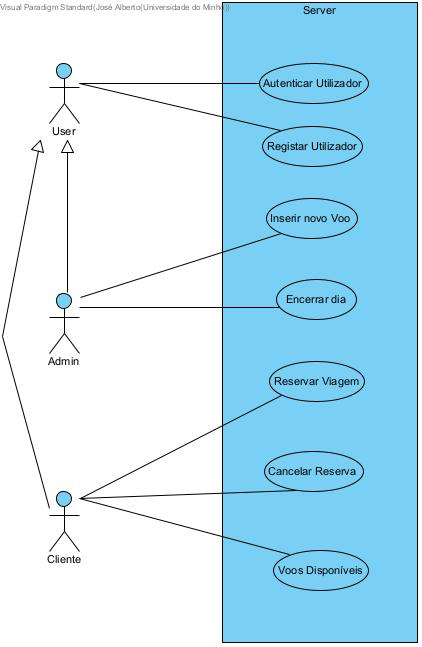
\includegraphics[width=0.5\textwidth]{diagrams/Server Use Case Diagram.jpg}
    \caption{Diagrama de Use Cases do \textit{Flight Manager}}
\end{figure}

A partir das funcionalidades mencionadas no enunciado do trabalho proposto, foram distribuídas as opções para os
utilizadores da aplicação, seguindo a conceção do sistema.

Esta, divide-se em três grandes componentes:
\begin{itemize}
    \item[Cliente]{Responsável pela apresentação e envio dos pedidos disponíveis do Cliente.}
    \item[Servidor]{Responsável pela resposta por parte do Servidor.} 
    \item[Middleware]{Construtor das \textit{Querys} e \textit{Responses}, bem como gere o suporte para a conexão.} 
\end{itemize}

Considerou-se mais intuitivo previamente apresentar o modo como a conexão do Servidor/Cliente é geridas e o tipo
de mensagens criadas, sendo a primeira grande componente da aplicação a ser apresentada o: \textit{Middleware}.

\subsection{Middleware}
\subfile{middleware.tex}

\section{Cliente}
\subfile{cliente.tex}

\section{Servidor}
\subfile{servidor.tex}

\section{Funcionalidades Adicionais}

No seguimento da realização das funcionalidade obrigatórias pré-definidas pela equipa docente, 
foi considerada a adição de aspetos adicionais, de modo a enriquecer a resposta previamente 
construída.

\chapter{Considerações Finais}
\section{Conclusões}

Ao longo do desenvolvimento do projeto, e com o auxilio da equipa docente para qualquer questão 
relativa à matéria lecionada e à conceção do trabalho, o grupo foi munido com todos os conceitos
e materiais necessários para o bom desenvolvimento do sistema, \textit{Flight Manager}.

A partir de conceitos de outras unidades curriculares, o grupo foi possibilitado a resolver uma 
solução outrora complexa, a partir de um estruturamento planificado e modelado, usando para tal 
o sistema de modelação \textit{Visual Paradigm}.
Este permitiu, muito mais facilmente, fragmentar o que era necessário resolver para colocar o 
sistema a correr, poupando muito tempo que podia ser perdido, ao construir a aplicação "à mediada
que fazia".

O grupo encontra-se orgulhoso por poder implementar um sistema que não só responde às funcionalidades 
básicas estabelcidades pela equipa docente, com uma plataforma bem construída do ponto de vista
de encapsulamento e organização dos vários constituintes.

Escusado é dizer que muniu todos os participantes com experiência na realização de projetos que sigam 
os conceitos de \textbf{Sistemas Operativos}, nomeadamente a exclusão mútua, a programação com \textit{sockets} e
com várias \textit{Threads}.

\section{Trabalho Futuro}

Apesar de todo o processo de desenvolvimento do sistema \textit{Flight Manager} ter coincidido com as espectativas
colocadas pelo grupo, e, até permitido adicionar funcionalidades numa tentativa de obter um melhor aproveitamento,
existem alguns pontos que poderiam ser abordados numa iteração seguinte do \textbf{Flight Manager}.

Como qualquer sistema que visa a interação com utilizadores sem conhecimentos dentro da área de informática, o 
manuseamento de um terminal para utilizar a plataforma pode tornar-se incómodo.
Dado a aplicação querer satisfazer as necessidades de utilizadores comuns, seria de extrema importância a conceção
de uma interface com o utilizador intuitiva e simples de usar.
Assim, um dos problemas seria a criação de uma \textit{framework} conceptual para o \textbf{Flight Manager}.

Outra equívoco seria a adição de mais funcionalidades. 
O aperfeiçoamento da aplicação, de modo a chegar a um estado competitivo para o mercado atual, passaria pela
implementação de várias e diferentes funcionalidades que o distingue dos restantes produtos análogos.

%==========================================================================
% BEGIN LISTA DE SIGLAS E ACRÓNIMOS
%==========================================================================

%% Portuguese babel does not translate this environment
\renewcommand{\nomname}{Lista de Siglas e Acrónimos}

%% Text that can be shown before acronyms list
\renewcommand{\nompreamble}{}

%% acronyms
\nomenclature[01]{\textbf{SD}}{Sistemas Distribuídos}
\nomenclature[02]{\textbf{DTO}}{\textit{Data-Transfer Object}}
\nomenclature[03]{\textbf{UC}}{Unidade Curricular}
\nomenclature[04]{\textbf{plataforma}}{Sistema de gestão de reservas de voos}
\nomenclature[05]{\textbf{sistema}}{Sistema de gestão de reservas de voos}
\nomenclature[06]{\textbf{aplicação}}{Sistema de gestão de reservas de voos}
\nomenclature[06]{\textbf{programa}}{Sistema de gestão de reservas de voos}

%% Show acronyms
\printnomenclature

%==========================================================================
% END LISTA DE SIGLAS E ACRÓNIMOS
%==========================================================================

%==========================================================================
% BEGIN ANEXOS
%==========================================================================

\addchap{Anexos}

%==========================================================================
% END ANEXOS
%==========================================================================

\end{document}